\chapter{Solução Proposta}\label{cap:solucao}

Uma vez que o conhecimento teórico necessário para o entendimento completo do trabalho já foi apresentado, neste capítulo será definida a solução proposta.

A solução desenvolvida consiste em um algoritmo analisa imagens de vídeo de um estacionamento descoberto e determina o número de vagas livres na imagem, além da sua localização aproximada. O sistema funciona bem em imagens de menor qualidade, mas é necessário que o vídeo adquirido seja em cores.

O trabalho se preocupa em cumprir os critérios definidos no capítulo \ref{cap:trabalhos}. Além disso, o sistema foi desenvolvido de forma que pudesse processar as imagens adquiridas de forma mais próxima possível do tempo real, causando o mínimo de atrasos para o processamento de quadros subsequentes do vídeo.

O sistema recebe como entrada um vídeo em cores capturado em um certo ângulo e um vetor de regiões de interesse no vídeo. A saída do programa a cada quadro é o número de vagas livres em cada região de interesse no vídeo.

A imagem \ref{fig:fluxograma} contém um fluxograma que mostra as etapas do processamento de cada quadro do vídeo adquirido. No decorrer deste capítulo cada um desses passo será discutido com mais detalhes.

%%Fazer fluxograma e inserir aqui%%



\section{Aquisição}\label{sec:aquisicao}

Uma câmera montada em um poste de luz ou outro ponto similar captura as imagens utilizadas pelo programa. A câmera é montada de forma que o seu campo de visão contenha o máximo de vagas possível, porém que ainda seja possível visualizar o asfalto das vagas desocupadas e ocorra o mínimo de oclusão de veículos. A figura \ref{fig:aquisicao} mostra um quadro de uma aquisição em ângulo ideal.

\begin{figure}[!ht]
	\centering
	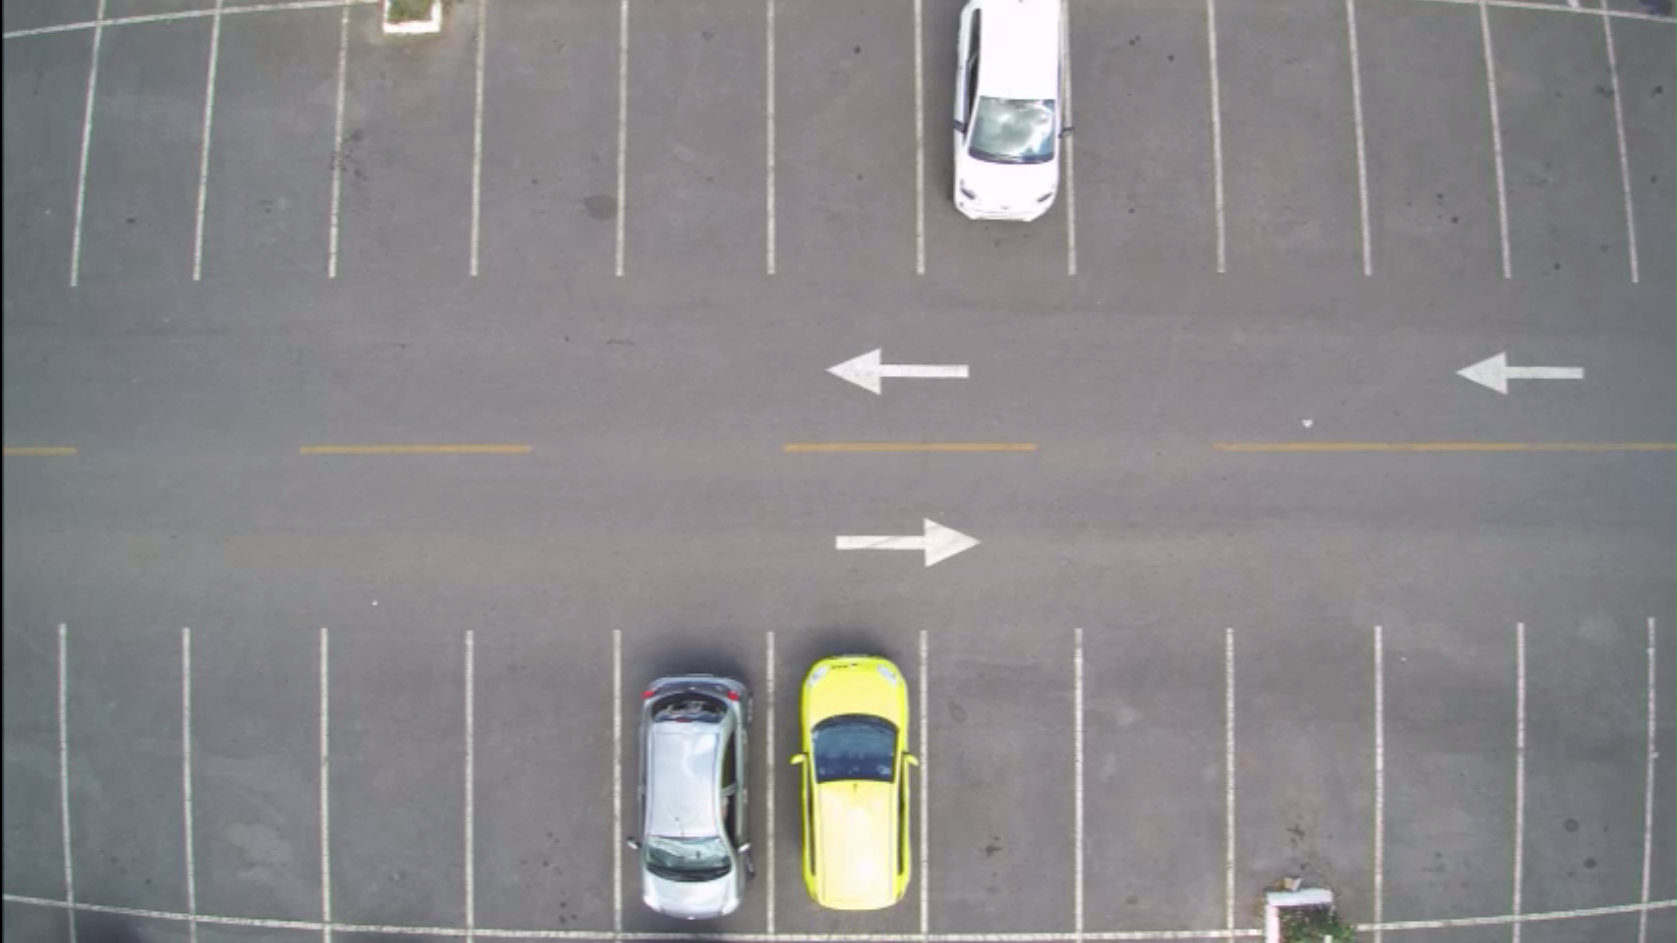
\includegraphics[width=8cm]{Vazio3}
	\label{fig:aquisicao}
	\caption{Um quadro de um vídeo adquirido por uma câmera do sistema}
	\centering
\end{figure}

Diversas câmeras podem ser instaladas para aumentar a cobertura do estacionamento. Neste caso, cada vídeo é processado por uma cópia diferente do sistema. Por isso, neste capítulo a discussão será focada apenas no processamento do vídeo de uma câmera.

\section{Regiões de Interesse}\label{sec:ROIs}

No momento da instalação do programa, é necessário definir um número qualquer de regiões de interesse(ROIs). Essas regiões determinam a área da imagem onde existem vagas. Além de determinar as regiões, deve-se informar ao programa o número de vagas existente em cada região de interesse.

As ROIs devem ser retangulares e determinadas de forma a não haver interseção entre elas, como exemplificado na figura \ref{fig:ROIs} que mostra as regiões determinadas para o quadro da figura \ref{fig:aquisicao}.

%Figura das regiões de interesse aqui %%

\section{Seções Verticais}\label{sec:secoesVerticais}

 





